\documentclass[a4paper, 12pt]{article}
\usepackage[english, russian]{babel}
\usepackage[utf8]{inputenc}
\usepackage[T2A]{fontenc}
\usepackage{verbatim}
\usepackage{amsmath, amsthm}
\usepackage{pdfpages}

\theoremstyle{plain}
\newtheorem{theorem}{Теорема}
\newtheorem{lemma}{Лемма}[theorem]

\theoremstyle{definition}
\newtheorem{definition}{Определение}

\theoremstyle{remark}
\newtheorem*{remark}{Замечание}

\setcounter{secnumdepth}{0}


\title{Конспект пары по <<Продвинутому ДП>>}
\author{Калмыков Андрей}
\date{2022}
\begin{document}
	\clearpage\maketitle
	\thispagestyle{empty}
	\newpage
	\tableofcontents
	\newpage
	\section{Первый день}
		Странно напоминать основы ДП людям пришедшим на продвинутое ДП, но пару слов об этом. Мы хотим решить задачу, разбив её на более простые подзадачи, зачастую пожертвовав памятью в угоду скорости. Есть $5$ пунктов, нужных для решения задачи по dp:
	\begin{enumerate}
		\item Что хранится в dp
	\item Формула пересчёта
	\item Порядок пересчёта
	\item База динамики
	\item Где лежит ответ
\end{enumerate}
	Есть базовые задачи и примеры вроде рюкзака, кузнечика, монеток и т.д. Их мы обсуждать не будем\\
	\subsection{НВП}
	Для начала разберём простенькую задачку о наибольшей возрастающей последовательности.\\
	\textit{Условие}:Дан массив из $n$ чисел $a[0\dots1]$. Требуется найти в этой последовательности строго возрастающую подпоследовательность наибольшей длины.\\
	\textit{Решение} за $O(n^2)$: Будем в $dp[i]$ хранить наибольшую длину возрастающей подпоследовательности на массиве $a[0\dots i]$, заканчивающейся в $a[i]$. \\
	База: $dp[0]=a[0]$\\
	Переход $dp[i] =\max( \max\limits_{j<i, a_j<a_i}(1+dp[j]),1)$\\
	Переход корректен, так как мы просто продляем предыдущую наибольшую с элементом поменьше следующим. Так как мы проходимся по всем элементам, и для каждого элемента проходимся по всем предыдущим, то и асимптотика будет $O(n^2)$ врмени и $O(n)$ памяти\\
	Код:
	\begin{verbatim}
		dp[0] = 0
		for i = 1...n
		    dp[i] = 1
		    for j = 1...i - 1
		        if (a[j] < a[i])
		            dp[i] = max(dp[i], 1+dp[j])
	\end{verbatim}
Ответ: $\max(dp[1],\dots,dp[n])$\\
\begin{remark}
	Другое решение за $O(n^2)$.\\
	Пусть $b$ --- отсортированное $a$. Тогда $|\text{НВП}(a)|=|\text{НОП}(a,b)|$\\
	А так как у нас \textit{НОП} считается за квадрат, то и конечная асимптотика будет таковой
\end{remark}
\textit{Решение1 за} $O(n\log n)$:  заметим, что если числа обновляются, то они увеличиваются, кроме того нам надо находить максимум. Это приводит нас к идее дерева отрезков или дерева Фенвика, так как нам нужны операции обновления в точке (только увеличения) и максимума на отрезке.\\
Сначала "убьём" все элементы. Будем оживлять их в порядке возрастания. Когда мы оживляем $i$-ый элемент, то все меьшие его уже оживлены, а значит нам нужен максимум $dp$ gо живым элементам на отрезке $[0\dots i]$\\
Для удобства считаем, что числа попарно различны, иначе оживляем одинаковые справа налево.\\
Пусть $a_{k_1}<a_{k_2}<\dots<a_{k_n}$\\
Заводим дерево Фенвика на $[0,n]$, заполняем $-\infty$\\
\begin{verbatim}
	for i = 1...n
	    x = get(1, k_i - 1)
	    upadte(k_1, max(1, 1 + x))
\end{verbatim}
Мы перебираем все $n$ элементов, при этом из-за асимптотики операций в дереве Фенвика мы получим асимптотику $O(n\log n)$ по времени и $O(n)$ по памяти\\
Ответ: $\max(dp[i])$\\
\textit{Решение2 за} $O(n\log n)$: теперь мы переработаем решение так, чтобы было достаточно бинарного поиска.\\
Пусть $dp[i][k]$ "--- это минимальный последний элемент в ВП длины $k$ массива $a_1,\dots,a_i$ (или $+\infty$, если такой ВП нет). Тогда мы можем сделать последовательность дилны $k$ на массиве $a[0\dots i]$, кончающуюся в $a[i]$, если на массиве $a[0\dots i-1]$ есть последовательность длины $k-1$, заканчивающаяся на меньший элемент.\\
Заметим, что $dp[i][*]$ возрастает.\\
Докажем, что $dp[i][k]<dp[i][k+1]$. Рассмотрим $x=dp[i][k+1]$, заметим, что предпоследний элемент этой последовательности очевидно является кандидатом на $dp[i][k]$, также он меньше $x$, а значит доказываемое выполняется.\\
Рассмотрим переход $dp[i][\cdot]\to dp[i+1][\cdot]$.\\
$dp[i+1][k] = a_{i+1} \text{ или } dp[i][k]$. То есть, если представить $dp$ как таблицу, то в следующей строке часть значений будут перекопированы, а часть изменены, но так как массив возрастает, то поменяется максимум одно значение. Если их $2$, то невозрастающий массив. Далее рассматриваем пример работы алгоритма на  $dp[i]=\{1,3,5,6,10,12, +\infty\}, a[i+1]=7\Rightarrow dp[i+1]=\{1,3,5,6,7,12,+\infty\}$.\\
Тогда в итоге алгоритм таков: на каждом шаге находим больший элемент в $dp$ и заменяем его на новый элемент, если новый больше всех, то ставим его в конец. Больший элемент ищем бинпоиском. Отсюда и асимптотика по времени $O(n\log n)$ и по времени $O(n)$.\\
Ответ: $\max\limits_{dp[n][k]\not=+\infty}k$
\subsection{Графы и возведение матриц в степень}
Так как нахождению рекурент, а следовательно и возведению матриц в степень вас в случае чего научат на другой паре в будущем, то я лишь кратенько напомню, что найти $n$-ую степень матрицы можно за $O(k^3\log n)$, умножая матрицы за куб и пользуясь бинарным возведением в степень.\\
\textit{Условие1:} Найти кол-во путей из $u$ в $v$ длины ровно $k$ (считаем $\% m$)\\
Пусть $M$ "--- матрица смежности графа, т.е. $M_{ij}=\begin{cases}
	1, &\text{если есть ребро из }i \text{ в } j\\
	0, &\text{иначе}
\end{cases}$
Тогда мы утверждаем, что $(M^k)_{ij}$ "--- число путей из $i$ в $j$ длины ровно $k$
\begin{proof}
	Индукция по $k$\\
	$k=1$ --- очевидно, наличие пути аналогично наличичию ребра\\
	Пусть верно для $(k-1)$\\
	$(M^k)_{ij}=(M\cdot M^{k-1})_{ij}=\sum\limits_{t=1}^nM_{it}\cdot (M^{k-1})_{tj}$ --- тут мы перым шагом идём из $i$в $t$, а потом за оставшиеся $k-1$ шагов пытаемся попасть из $t$ в $j$, а так как предположение индукции верно, то всё работает
\end{proof}
Также данное решение с лёгкостью перекладывается на мультиграф, просто вместо единицы в матрице смежности будет число рёбер из $i$ в $j$.\\
\textit{Условие2:} Число путей из $i$ в $j$ длины $\leq k$.\\
По сути нам надо вычислить $\left(\sum\limits_{t=0}^kM^t\right)_{ij}=:A_k$\\
Заметим, что $A_k=A_{\frac{k}{2}}+M^{\frac{k}{2}}\cdot A_{\frac{k}{2}}=\left(E+M^{\frac{k}{2}}\right)\cdot A_{\frac{k}{2}}$ --- отсюда мы получаем рекурсию, которую считаем при помощи бинарного возведения в степени. (В принципе мы можем завести $2$ вспомогательные функции, одну для счёта степени, другую --- для суммы)\\
Итоговая асимптотика: $O(n^3\log k)$\\
\textit{Условие3:} Есть ли путь из $i$ в $j$ длины $k$?\\
Теперь покажем, как можно решить, переопределив умножение матриц.\\
Пусть $M$ "--- матрица смежности\\
$(M\odot M\odot\dots\odot M)_{ij}=\begin{cases}
	1, &\text{если есть путь, удовлетворяющий условию}\\
	0, &\text{иначе}
\end{cases}$
Пусть $A\odot B=C: c_{ij}=\bigvee\limits_t(a_{it}\wedge b_{tj})$\\
Точно также индукцией по $k$ можно показать, что $(M^{\odot k})_{ij}$ --- ровно то, что нужно\\
Факт (б/д): для возможности применения бинарного возведения в степень достаточно ассоциативности нашего умножения\\
А сама ассоциативность доказывается аналогично ассоциативности обычного умножения
\section[ДЗ1]{Первая домашка}
Тут случайно затесалась ещё одна задачка, но в первую домашку идёт только первые $2$
%\includepdf[pages={7-8}]{Algo_Th_Kalmykov.pdf}
\section{Второй день}
\subsection{ДП по маскам(по подмножествам)}
Пусть есть небольшое множество $A=\{0,1,2,\dots,n-1\}$, мы хотим как можно более эффективно представлять его подмножества. Пусть $n\leq30$. Будем кодировать подмножества с помощью битовых строк длины $n$, т.е. подмножество $A\leftrightarrow$ битовые строки длины $n$. Тогда мы просто интерпретируем строку как число в двоичной системе счисления.\\
Теперь хотим научиться делать некоторые операции над маскаи:
\begin{enumerate}
	\item Извлечение бита, проверка наличия элемента в множестве:
	\begin{verbatim}
		bool bit(int mask, int pos){
		    return (mask >> pos) & 1; 
	}
	\end{verbatim}
\item Объединение множеств: $A\cup B=mask_A | mask_B$
\item Пересечение множеств: $A\cap B =mask_A \& mask_B$
\item Разность множеств, есть разные способы, мы будем использовать: $A\backslash B=(mask_A | mask_B) \wedge mask_B$
\end{enumerate}
\textit{Задача 1} Дан полный вхвешенный граф, найти самый дешёвый гамильтонов путь, т.е. все вершины посетить по одному разу. В такой постановке эта задача $NP$-трудная (нет решения за полином), поэтому будем решать за экспоненту.\\
Идея, для каждого пути, чтобы знать, куда пойти, достаточно хранить последнюю вершину и список посещённых\\
Пусть $dp[v][mask]$ "--- мин вес пути, который заканчивается в $v$ и посещает все вершины из $mask$ по одному разу\\
База: $\forall dp[v][2^v]=0;\\
dp[\cdot][v]=+\infty$\\
Переход, ДП вперёд: 
\begin{verbatim}
	for u=0...n - 1
	    if (!bit(mask, u))
	        new_mask = mask | (1 << u)
	        dp[u][new_mask] = min(dp[u][new_mask], dp[v][mask] + cost[v][u])
\end{verbatim}
\newpage
Порядок пересчёта: надо перебирать маски в порядке включения, то есть для каждой маски перебираем надмножества, т.е. перебираем маски в порядке возрастания:
\begin{verbatim}
	for mask = 0...2^n - 1
	    for v = 0...n - 1
\end{verbatim}
Очевидно, что тогда мы переберём все подмножества до входа в маску, значит порядцок пересчёта будеи корректен\\
Асимптотика очевидно получается $O(2^n\cdot n^2)$ времени и $O(2^n\cdot n)$ памяти.
Ответ: $\min\limits_vdp[v][2^n-1]$\\
\textit{Задача 2:} Дан граф. Найти в нём максимальную клику, т.е. клику, содержащую максимальное количество вершин. Это тоже $NP$-трудная задача\\
\textit{Решение 1:} $O(2^n\cdot n^2)$ "--- полный перебор всех подмножеств\\
\textit{Решение 2:} $dp[mask]=\begin{cases}
	true, &\text{mask "--- клика}\\
	false, &\text{иначе}
\end{cases}$\\
Пусть $v\in mask$, тогда $dp[mask]=true\Leftrightarrow\begin{cases}
	dp[mask\textasciicircum2^v]=true\\
	v\text{ соединена со всеми из }(mask\textasciicircum2^v)
\end{cases}$\\
Данное условие проверяется за $O(n)\Rightarrow$ итоговая асимптотика $O(2^n\cdot n)$\\
\textit{Решение 3:} Можем вместо одной вершины откучывать по $2$вершины, тогда переход будет за $O(1)$, что даст решение за $O(1)$\\
\textit{Решение 4:} Давайте считать, что $v$ "--- старший бит в маске:
\begin{verbatim}
	int oldest = -1
	for mask = 1...2^n - 1
	    if (!(mask & (mask - 1))){
	        ++oldest
    }
\end{verbatim}
Используем $oldest$ вместо $v$\\
Осталось понять, соединён ли $oldest$ с остальными вершинами $mask$. Для каждой вершины $u$ изначально найдём маску всех её соседей $neighbor[u]$\\
$v$ соединена со всеми из $mask'\Leftrightarrow mask'\subset neighbor[v]\Leftrightarrow(mask'\backslash neighbor[v])=0$\\
Получили решение за $O(2^n)$\\
\textit{Решение 5(meet in the middle):} за $O(2^{\frac{n}{2}}\cdot n)$\\
Разобьём исходное множество на $2$ множества размером $\frac{n}{2}$. Тогда клика в исходном графе состоит из клики в первом множестве и клики во втором множестве, таких что каждая вершина из первой клики соединена с вершиной из второй.\\
Давайте переберём все клики в левом подмножестве, а для каждой клики будем из множества вершин, каждая из которых соединена со всеми вершинами клики, выбирать максимальную клику. Останется найти такой момент, когда сумма мощностей обеих клик максимальна.\\
Заведём $dp'[U]$ "--- маска вершин правой доли, каждая из которых соединена со всеми вершинами из $U$, $dp''[W]$ "--- размер макс подклики в маске $W$(правая доля)\\
Пусть слева $N$ вершин, справа --- $M$\\
$dp'[0]=2^M-1\\
dp'[mask]=dp'[mask\textasciicircum 2^{oldest}] \& neighbor[oldest]\\
dp''[mask]=\max\{|submask|:submask\text{ образует клику в правой доле, }submask\subset mask\}\\
a(mask)=\begin{cases}
	0, &mask\text{ не клика}\\
	|mask|, &\text{иначе}
\end{cases}\\
dp''[mask]=\max\limits_{submask\subset mask}a(submask)\\
b[k][mask]=\max\limits_{submask\subset mask\text{, submask и mask совпадают в старших k битах}}a(submask)\\
b[M][mask]=a(mask)$ \\
Рассматриваем $k$-ую степень свободы:\\
\begin{verbatim}
	if (!bit(mask, M - k))
	    b[k - 1][mask] = b[k][mask]
	else
	    b[k - 1][mask] = max(b[k][mask], b[k][mask^(2^(M-k))])
\end{verbatim}
Ответ: $dp''[mask]=b[0][mask]$\\
\textit{Решение 6:} за $O(2^{\frac{n}{2}})$. Это более частный случай, но в данном случае асимптотика улучшается. $dp''[mask]=\max(dp''[mask\textasciicircum2^{oldest}], 1+dp''[mask\&neighbor[oldest]])$
\subsection{ДП по профилю}
Пусть имеется клеточная табличка $m\times n$, хотим узнать количество способов замостить её вертикальными и горизонтальными доминошками. Вообще эта задача не $NP$-трудная, т.е. существует явная формула для подсчёта при фиксированных $n$, но мы научимся считать за экспоненту при маленьких значениях. Самая простая динамика не подойдёт, ведь будут вылезающие горизонтально доминошки, поэтому мы запомним, где они вылезают и номер столбца:\\
$dp[j][mask]$ --- хотим зафиксировать\\
Хотим $(j, mask_1)\to(j+1,mask_2)$. Занесём в $mask$ торчащие вправо доминошки, тогда то, что не замостилось торчащими слева и справа надо замостить вертикальными доминошками. Такое покрытие либо одно, либо их нет. Тогда если мы напишем процедуру, проверяющую, можно ли замостить стобец, то мы сможем проверить возможность перехода между масками.\\
$dp[j+1][mask_2]+=dp[j][mask_1]$, если возможно\\
База и ответ очевидны, а асимптотика $O(4^n(n+m))$
\section[ДЗ 2]{Вторая домашка}
%\includepdf[pages={8-10}]{Algo_Th_Kalmykov.pdf}
\section{Третий день}
\subsection{ДП на подотрезках}
Для демонстрации принципов работы ДП на подотрезках рассмотрим задачку про нахождение наибольшего палиндрома в строке. Эта задача или подобная ей встречалась на межнаре 2000 года. Формально звучит она так: имеется строка $S$, найдите палиндром наибольшей длины.\\
\textit{Наивное неправильное решение}: Попробуем вычислить $ans[i]$ "--- длина наибольшего палиндрома подстроки $s$, содержащей только первые $i$ символов. Заметим, что если последний символ не входит в палиндром, то мы просто берём $ans[i-1]$, иначе же мы ищем первый символ, совпадающий с последним, но вот незадача --- как нам посчитать длину палиндрома на этом отрезке?\\
Тут то и надо понять, что стоит воспользоваться динамикой по подотрезкам: давайте хранить в $dp[l][r]$ длину наибольшего палиндрома на отрезке $[l,r]$\\
База: $dp[l][l]=1$\\
Переход: $dp[l][r]=\begin{cases}
	\max(dp[l+1][r], dp[l][r-1]), &S[l]\not=S[r]\\
	dp[l+1][r-1]+2, &S[l]=S[r]
\end{cases}$\\
Порядок пересчёта: тут нас поджидает ещё одна проблема, просто пробегаться $l$ по всему массиву, а $r$ по оставшейся части не сработает, так как нам требуется  $l+1$, поэтому будет пробегаться вначале по длине подотрезка, а потом по его началу:
\begin{verbatim}
	for len = 1...n
	    for l = 1...n - len + 1
	        r = l + len - 1
	        dp[l][r] = ...
\end{verbatim}
Ответ: ответ будет лежать в $dp[0][n-1]$\\
Асимптотика: так как мы имеем два вложенных цикла, то работает наше чудо за $O(n^2)$\\
Итоговая идея заключается в том, что мы просто решаем задачу на меньших подотрезках, а потом из них получаем большие, иногда, кстати, полезно склеивать подотрезки.
\subsection{Метод четырёх русских}
Для начала давайте разберёмся с методом и задачей, а потом подумаем, в каких местах это может быть полезно\\
\textit{Условие:} Пусть имеется две матрицы размерами $n\times n$, состоящие из нулей и единиц. НУжно найти их произведение по модулю $2$.\\
\text{Наивное решение:} мы можем просто втупую перемножить матрицы по определению: $C=A\cdot B \Leftrightarrow \left(c_{ij}=\sum\limits_{k=1}^na_{ik}\cdot b_{kj}\right)$. Но сложность алгоритма тогда будет $O(n^3)$. Попробуем улучшить это время\\
\textit{Сжатие матриц:} для выполнения сжатия матриц выполним следующий предподсчёт : для всех возможных пар двоичных векторов длины $k$ подсчитаем и запомним их скалярное произведение по модулю $2$.\\
Возьмём первую матрицу. разделим каждую её строку на куски размера $k$. Для каждого куска определим номер двоичного вектора, который соответствует числам, находящимся на этом куске. Если кусок получился неравным по длине $k$ (последний кусок строки), то будем считать, что в конце в нём идут не влияющие на умножение нули. Получим матрицу $A'_{n\times\lceil\frac{n}{k}\rceil}$.\\
Аналогично поступим с матрицей $B$, вместо строк деля столбцы. Получим матрицу $B'_{n\times\lceil\frac{n}{k}\rceil}$.\\
Теперь, если вместо произведения матриц $A$ и $B$ считать произведение новых матриц $A'$ и $B'$, воспользовавшись посчитанными скалярными произведениями, то каждый элемент матрицы C будет получаться уже за время, пропорциональное $\lceil\frac{n}{k}\rceil$ вместо $n$, и время произведения матриц сократится с $O(n^3)$ до $O(n^2\cdot \frac{n}{k})=O(\frac{n^3}{k})$.\\
Теперь оценим сложность алгоритма и выберем оптимальное $k$:
\begin{itemize}
	\item Предподсчёт происходит за $O(2^{2k}k)$
	\item Сжатие матриц происходит за $O(n^2)$
	\item Перемножение сжатых матриц происходит за $O(\frac{n^3}{k})$
\end{itemize}
Итого: $O(2^{2k}k)+O(\frac{n^3}{k})$. Выбрав $k=\log n$, получим оптимальную асимптотику:
\[O(n^2\log n)+O(\frac{n^3}{\log n})=O(\frac{n^3}{\log n})\]
Далее приводим пример перемножения двух матриц этим методом.\\
Кстати, метод четырёх русских с некоторыми модификациями можно применить к НОП для получения небольшого выигрыша
\subsection{Convex hull trick}
\begin{definition}
	Convex hull trick "--- один из методов оптимизации динамического программирования, использующий идею выпуклой оболочки. Позволяет улучшить асимптотику некоторых задач, решаемых методом динамического программирования с $O(n^2)$ до $O(n\log n)$
\end{definition}
Рассмотрим задачу, где этот трюк можно применить:\\
\textit{Условие:} Есть $n$ деревьев с высотами $a_1,a_2,\dots,a_n$ (в метрах). Требуется спилить их все, потратив минимальное количество монет на заправку бензопилы. Но пила устроена так, что она может спиливать только по $1$ метру от дерева, к которому ее применили. Также после срубленного метра (любого дерева) пилу нужно заправлять, платя за бензин определенное кол-во монет. Причем стоимость бензина зависит от срубленных (полностью) деревьев. Если сейчас максимальный индекс срубленного дерева равен $i$, то цена заправки равна $c_i$. Изначально пила заправлена. Также известны следующие ограничения : $c_n=0,a_1=1,a_i$ возрастают, $c_i$ убывают. Изначально пила заправлена.\\
\textit{Наивное решение}: Сначала заметим важный факт : т.к. $c[i]$ убывают (нестрого) и $c[n]=0$, то все $c[i]$ неотрицательны. Понятно, что нужно затратив минимальную стоимость срубить последнее ($n$-е) дерево, т.к. после него все деревья можно будет рубить бесплатно (т.к. $c[n]=0$). Посчитаем следующую динамику : $dp[i]$ — минимальная стоимость, заплатив которую можно добиться того, что дерево номер $i$ будет срублено. База динамики : $dp[1]=0$, т.к. изначально пила заправлена и высота первого дерева равна $1$, по условию задачи. Переход динамики : понятно, что выгодно рубить сначала более дорогие и низкие деревья, а потом более высокие и дешевые (док-во этого факта очевидно). Поэтому перед $i$-м деревом мы обязательно срубили какое-то $j$-е, причем $j\leq i-1$. Поэтому чтобы найти $dp[i]$ нужно перебрать все $1\leq j\leq i-1$ и попытаться использовать ответ для дерева номер $j$. Итак, пусть перед $i$-м деревом мы полностью срубили $j$-е, причем высота $i$-го дерева составляет $a[i]$, а т.к. последнее дерево, которое мы срубили, имеет индекс $j$, то стоимость каждого метра $i$-го дерева составит $c[j]$. Поэтому на сруб $i$-го дерева мы потратим $a[i]\cdot c[j]$ монет. Также не стоит забывать, что ситуацию, когда $j$-е дерево полностью срублено, мы получили не бесплатно, а за $dp[j]$ монет. Итоговая формула пересчета : $dp[i]=\min\limits_{j=1\dots i-1}(dp[j]+a[i]\cdot c[j])$.\\
Такое решение очевидно будет работать за $O(n^2)$
\textit{Ключевая идея оптимизации:} Для начала сделаем замену обозначений. Давайте обозначим $dp[j]$ за $b[j]$, $a[i]$ за $x[i]$, а $c[j]$ за $k[j]$.\\
Теперь формула приняла вид $dp[i]=\min\limits_{j=0\dots i-1}(k[j]\cdot x[i]+b[j])$. Выражение $k[j]\cdot x+b[j]$ "--- это в точности уравнение прямой вида $y=kx+b$.
Сопоставим каждому $j$, обработанному ранее, прямую $y[j](x)=k[j]\cdot x+b[j]$. Из условия «$c[i]$ убывают $\Leftrightarrow k[j]$ уменьшаются с номером $j$» следует то, что прямые, полученные ранее отсортированы в порядке убывания углового коэффициента. Давайте нарисуем несколько таких прямых *пример*\\
Выделим множество точек $(x_0,y_0)$ , таких что все они принадлежат одной из прямых и при этом нету ни одной прямой $y'(x)$, такой что $y'(x_0)<y_0$. Иными словами возьмем «выпуклую (вверх) оболочку» нашего множества прямых (её еще называют нижней огибающей множества прямых на плоскости). Назовем ее <<$y=convex(x)$>>. Видно, что множество точек $(x,convex(x))$ представляет собой выпуклую вверх функцию.
\textit{Цель нижней огибающей множества прямых:} Пусть мы считаем динамику для $i$-го дерева. Его задает $x[i]$. Итак, нам нужно для данного $x[i]$ найти $\min\limits_{j=0\dots i-1}(k[j]\cdot x[i]+b[j])=\min\limits_{j=0\dots i-1}(y[j](x[i]))$. Это выражение есть $convex(x[i])$. Из монотонности угловых коэффицентов отрезков, задающих выпуклую оболочку, и их расположения по координатам $x$ следует то, что отрезок, который пересекает прямую $x=x[i]$, можно найти бинарным поиском. Это потребует $O(\log n)$ времени на поиск такого $j$, что $dp[i]=k[j]\cdot x[i]+b[j]$. Теперь осталось научиться поддерживать множество прямых и быстро добавлять $i$-ю прямую после того, как мы посчитали $b[i]=dp[i]$.\\
Воспользуемся идеей алгоритма построения выпуклой оболочки множества точек. Заведем $2$ стека $k[]$ и $b[]$, которые задают прямые в отсортированном порядке их угловыми коэффицентами и свободными членами. Рассмотрим ситуацию, когда мы хотим добавить новую ($i$-тую) прямую в множество. Пусть сейчас в множестве лежит $sz$ прямых (нумерация с $1$). Пусть $(x_L,y_L)$ "--- точка пересечения $sz-1$-й прямой множества и $sz$-й, а $(x_R,y_R) $ "--- точка пересечения новой прямой, которую мы хотим добавить в конец множества и $sz$-й. Нас будут интересовать только их $x$-овые координаты $x_L$ и $x_R$, соответственно. Если оказалось, что новая прямая пересекает $sz$-ю прямую выпуклой оболочки позже, чем $sz$-я $sz-1$-ю, т.е.$ (x_L\geq x_R)$, то $sz$-ю удалим из нашего множества, иначе - остановимся. Так будем делать, пока либо число прямых в стеке не станет равным $2$, либо $x_L$ не станет меньше $x_R$.\\
Асимптотика : аналогично обычному алгоритму построения выпуклой оболочки, каждая прямая ровно $1$ раз добавится в стек и максимум $1$ раз удалится. Значит время работы перестройки выпуклой оболочки займет $O(n)$ суммарно.
\section{Четвёртый день}
\subsection{Корректность алгоритма построения нижней огибающей множества прямых сторон}
\begin{proof}
	Достаточно показать, что последнюю прямую нужно удалить из множества $\Leftrightarrow$, когда наша новая прямая пересекает её в точке с координатой по оси $X$, меньшей, чем последняя --- предпоследнюю.\\
	Пусть $Y(x)=Kx+B$ "--- уравнение новой прямой, $y[i](x)=K[i]x+B[i]$ "--- уравнения прямых множества. Тогда так как $K<K[sz]$, то при $x\in[-\infty;x_R]:y[sz](x)\leq Y(x)$, а так как $K[sz]<K[sz-1]$, то при $x\in[x_L;+\infty]:y[sz-1](x)\geq y[sz](x)$. Если $x_L<x_R$, то при $x\in[x_L;x_R]:y[sz-1]\geq y[sz](x)$ и $Y(x)\geq y[sz](x)$, т.е. на отрезке $[x_L;x_R]$ прямая номер $sz$ лежит ниже остальных и её нужно оставить в множестве. Если же $x_L > x_R$, то она ниже всех на отрезке $[x_L;x_R]=\emptyset$, т.е. её можно удалить из множества
\end{proof}
Из-за того, что условие на убывание/возрастание встречается нечасто, то зачастую приходится применять динамическую версию этого трюка. Вкратце, тут помогает двоичное дерево поиска.
\subsection{Графы. 2SAT}
ДП и графы уже давно крепко сплелись во многих местах, так что в рамках этой и следующей пары мы будет говорить о графах. Я не буду рассказывать самую базу вроде алгоритмов обхода, поиска компонент связанности, а также алгоритмы Дейкстры и Прима. Но поговрю о применениях этих алгоритмов и о более сложных и изощрённых алгоритмах.\\
И начнём мы с 2SAT: пусть мы имеем $\varphi$ "--- формулу в 2КНФ "--- конъюнкция (И) некскольких скобок, каждая скобка --- дизъюнкция (ИЛИ) ровно двух литералов ($p/\bar{p}$)\\
Цель: найти выполняющий набор для формулы $\varphi$ ил сказать, что его нет.\\
Решение: для каждой переенной заведём две вершины: $x\to x,\bar{x}$. Каждую скобку превратим в $2$ ребра, так как $(x\vee y)=(\neg x\rightarrow y) = (\neg y \rightarrow x)$ *рисуем примерчики и объясняем, какие рёбра проводим*\\
\textbf{Утв} $\varphi$ выполнима $\Leftrightarrow \not\exists p:p$ и $\neg p$ лежат в одной КСС (компоненте сильной связанности)
\newpage
\begin{proof}
	$\text{ }$
	\begin{itemize}
		\item[$\Rightarrow$]Предположим противное, т.е. $p,\neg p\in$ одной КСС, в импликацию мы вкладывали следующий смысл: <<Если верно нчало стрелочки, то верен и конец>>, но в КСС обяхательно есть единица, иначе не верна формула, но тогда $p=\neg p$ --- противоречие
		\item[$\Leftarrow$] Пусть алгоритм Косарайю для каждой вершины сохраняет номер её КСС ($v\to C(v)$). Тогда $\forall p\hookrightarrow C(p)\not=C(\neg p)$\\
		Тогда скажем, что \begin{align*}
			p=1&\Leftrightarrow C(p)>C(\neg p)\\
			p=0&\Leftrightarrow C(p)<C(\neg p)
		\end{align*}
		Покажем, что это выполняющий набор. Пусть это не так, т.е. $\exists (x\vee y)=0 \Rightarrow x=y=0 \Rightarrow C(x)<C(\neg x) \&\& C(y)<C(\neg y)$. Но эта скобка присутствует в исходной формуле, а значит существуют два ребра: $\neg x\to y; \neg y\to x$.\\
		Заметим следующее: $C(\neg x)\leq C(y), C(\neg y)\leq C(x)$ (здесь рисуночек рисуем), отсюда следует противоречие, если расписать неравенства
	\end{itemize}
\end{proof}
Заметим, что алгоритм Косарайю и алгоритм 2SATработают за линию, так как основаны на DFS
\subsection{Мосты и их поиск}
\begin{definition}
	Пусть $G$ "--- связный граф. Тогда ребро $e$ называется мостом, если $G-e$ несвязный
\end{definition}
\textit{Цель:} хотим найти в графе все мосты\\
Введём $ret[v]=\min(tin[v], \min\limits_{(w,u) \text{ "--- обр. ребро, w в поддереве v}}tin[u])$.  Фактически $ret$ "--- это наиболее высокая веришна, куда мы можем попасть из какой-то вершины поддерева за $1$ шаг.\\
\textbf{Утв} древесное ребро $e=(v, to)$ является мостом $\Leftrightarrow ret[to]=tin[to]$
\begin{proof}
	Недревесные рёбра мостами быть не могут, так как их удаление не влияет на связность.
	\begin{itemize}
		\item[$\Leftarrow$] Если $ret[to]=tin[to]$, то после удаления ребра $(v, to)$ не будет пути между $v$ и $to$
		\item[$\Rightarrow$] Пусть $ret[to]<tin[to]$. Тогда после удаления $(v, to)$ по-прежнему будет путь из $to$ в $v$, значит граф по-прежнему связен, значит $e$ не мост
	\end{itemize}
\end{proof}
Теперь покажем, как это выглядит в коде:
\begin{verbatim}
	void dfs(int v, int p = -1){
	    parent[v] = p; fin[v] = timer++;
	    ret[v] = tin[v]; used[v] = true;
	    for (int to:g[v]){
	        if (to == p) continue;
	        if (used[to]) ret = min(ret[v], tin[to]);
	        else{
	            dfs(to, v);
	            ret[v] = min(ret[v], ret[to]);
	            if (ret[to] == tin[to]) => (v, to) - мост
        }
    }
}
\end{verbatim}
Докажем корректность, т.е. к моменту выхода из $v$ корректно насчитано $ret[v]$: доказываем индукцией по глубине спуска, так как в детях считаем корректно, то и в родителях тоже.
\section{Пятый день}
\subsection{Алгоритм A*}
\begin{definition}
	Находит расстояние от $s$ до $t$. Отличием от Дейкстры является то, что в Дейкстре мы выбирали следующую вершину основываяюсь лишь на растоянии до стартовой, но теперь мы хотим делать оценку на расстояние до конца, тем самым в реальности улучшая эффективность (на деле же асимптотика не отличается)\\
	Заведём $3$ функции:
	\begin{itemize}
		\item $g(v)$ "--- текущее найденная оценка на $dist(s,v)$
		\item $h(v)$ "--- оценка на $dist(v, t)$
		\item $f(v)=g(v)+h(v)$
	\end{itemize}
Грубо говоря, $A*$ "--- алгоритм Дейкстры на значениях $f$
\end{definition}
\begin{verbatim}
vector<double> g;
vector<double> f;
priority_queue q; --- куча номеров вершин, упорядоченных по f
g[s] = 0; f[s]=h(s);q.insert(s);
while(true){
    int v = q.extractMin();
    for (edge e:graph[v]){
        x = g[v] + e.cost;
        if (g[e.to] > x){
            g[e.to] = x;
            f[e.to] = g[e.to] +h(e.to);
            если e.to находится в q, то decreaseKey, иначе insert
    }
}
}
\end{verbatim}
\begin{definition}
	Функция $h$ (называемая эвристикой) называется допустимой, если $\forall v: 0\leq h(v)\leq dist(v, t)$
\end{definition}
\begin{definition}
	Эвристика $h$ называется монотонной, если $\forall (u,v): h(u)\leq h(v) + e.cost; h(t)=0$
\end{definition}
\begin{remark}
	Очевидно, что монотонная эвристика является допустимой
\end{remark}
\begin{theorem}
	Без доказательства. 
	\begin{enumerate}
		\item Если $h$ "--- монотонная эвристика, то $A*$ всегда вернёт правильный ответ, при этом каждая вершина раскроется $\leq1$ раза
		\item Если $h$ "--- допустимая, то $A*$ всегда вернёт правильный ответ, но в худшем случае за экспоненциальное время (это хорошо с точки зрения получения ответа, но непрактично с тз времени работы)
		\item Если $h$ "--- недопустимая, то $A*$ может вернуть хорошее приближение к ответу, но в худшем случае неверный ответ за экспоненциальное время (так как $A*$ используется в играх, то вполне приемлимо ошибаться, главное, что работает быстро)
	\end{enumerate}
\end{theorem}
\begin{proof}
	\textbf{Утв} Если $h$ "--- монотонная, то в $A*$ последовательность $f(v_1)\leq f(v_2)\leq\dots$ у извлекаемых вершин не убывает\\
	$f(to)$ могло не поменяться\\
	$f(to)=g(v)+e.cost+h(to)\leq f(v) = g(v) + h(v)\leq g(v) + h(to) + e.cost$ --- неравенство треугольника
	\newpage
	\textbf{Д-во теоремы пункт 1}  Вершина$v$ может быть извлечена дважды, только если $f(v)$ уменьшилось между извлечениями, что противоречит предыдущему утверждению\\
	Почему вернёт правильный ответ? $f(t)=g(t)$, т.к. $h(t)=0$\\
	Пусть алгоритм нашёл неоптимальный путь длины $f(t)$. Виртуально продолжим работу алгоритма, пока  $q$ не опустеет. Он найдёт $opt$, уменьшит $f(t)$, извлечёт $t$ с уменьшившимся значением, что противоречит утверждению
\end{proof}
Асимптотика $O(m\log n)$\\
В реальности асимптотика будет сильно лучше (пример с плоскостью и тем, что дейкстра будет расходитсья и расходиться, а $A*$ пойдёт в направлении конкретном)\\
Виды эвристик:
\begin{itemize}
	\item $h(v)=0\Rightarrow A*$ вырождается в алгоритм Дейкстры ($f=g$)
	\item $h(v)=dist(v,t)\Rightarrow A*$ рассмотрит почти только вершины на кратчайшем пути из $s$ в $t$. Идеальный случай
	\item Сетка с узлами, где можно двигаться только вверх, вниз, влево, вправо, тогда $h(v)=|v.x-t.x|+|v.y-t.y|$ "--- манхэттенское расстояние
	\item Если по той же клетчатой плоскости, но можем ходить и по диагонали, то хороша метрыка Чебышёва $h(v)=\max(|v.x-t.x|, |v.y-t.y|)$
	\item Евклидово расстояние, если мы просто на плоскости и можем ходить во все стороны $h(v)=\sqrt{(v.x-t.x)^2+(v.y-t.y)^2}$
\end{itemize}
\subsection{Алгоритм Флойда}
Алгоритм Флойда (алгоритм Флойда–Уоршелла) — алгоритм нахождения длин кратчайших путей между всеми парами вершин во взвешенном ориентированном графе. Работает корректно, если в графе нет циклов отрицательной величины, а в случае, когда такой цикл есть, позволяет найти хотя бы один такой цикл. Алгоритм работает за $\Theta(n^3)$ времени и использует $\Theta(n^2)$ памяти.
\textit{Описание} Обозначим длину кратчайшего пути между вершинами $u$ и $v$, содержащего, помимо $u$ и $v$, только вершины из множества $\{1\dots i\}$ как $d[u][v][i], d[u][v][0]=\omega_{uv}$ \\
На каждом шаге алгоритма, мы будем брать очередную вершину (пусть её номер --- $i$) и для всех пар вершин $u$ и $v$ вычислять $d[u][v][i]=\min(d[u][v][i-1],d[u][i][i-1]+d[i][v][i-1])$. То есть, если кратчайший путь из $u$ в $v$, содержащий только вершины из множества $\{1\dots i\}$, проходит через вершину $i$, то кратчайшим путем из $u$ в $v$ является кратчайший путь из $u$ в $i$, объединенный с кратчайшим путем из $i$ в $v$. В противном случае, когда этот путь не содержит вершины $i$, кратчайший путь из $u$ в $v$, содержащий только вершины из множества $\{1\dots i\}$ является кратчайшим путем из $u$ в $v$, содержащим только вершины из множества $\{1\dots i-1\}$\\
В коде просто перебираем $i, u, v$\\.
В итоге получаем, что матрица $d[*][*][n]$ и является искомой матрицей кратчайших путей, поскольку содержит в себе длины кратчайших путей между всеми парами вершин, имеющих в качестве промежуточных вершин вершины из множества $\{1\dots n\}$, что есть попросту все вершины графа. Такая реализация работает за $\Theta(n^3)$ времени и использует $\Theta(n^3)$ памяти.\\
Утверждается, что можно избавиться от одной размерности в массиве $d$, т.е. использовать двумерный массив $d_{uv}$. В процессе работы алгоритма поддерживается инвариант $r(u,v)\leq d_{uv}\leq d[u][v][i]$, а, поскольку, после выполнения работы алгоритма $r(u,v)=d[u][v][i]$, то тогда будет выполняться и $r(u,v)=d_{uv}$.\\
Для восстановления пути, нам нужно завести массив $next$, в который складывать вершину, если мы вдруг добавляем её в путь.\\
Для нахождения отрицательного цикла проверяем, произойдёт ли релаксация на следующем шаге
\section{Зачёт}
\subsection{Задача 1(2 балла)}
Вам требуется написать программу, которая по заданной последовательности находит максимальную невозрастающую её подпоследовательность (т.е такую последовательность чисел $a_{i_1},a_{i_2},\dots,a_{i_k} (i_1<i_2<\dots<i_k), что a_{i_1}\geq a_{i_2}\geq\dots\geq a_{i_k}$ и не существует последовательности с теми же свойствами длиной $k+1$).\\
\textbf{Решение} Мы создаём вектор из максимальных последних элементов, у последовательности
длины i, ветор хранящий номер элемента в исходной последовательности для
итоговой невозрастающей последовательности, а также номер в этом векторе для
предыдущего элемента, после чего идём по массиву, используя бинпоиск для
поиска, куда вставлять следующий, а также попутно заполняя массивы для
восстановления ответа. После чего мы идём по восстанавливающим ответ массивам и
восстанавливаем ответ.
\subsection{Задача 2(3 балла)}
Компания Gnusmas разработала новую модель мобильного телефона. Основное достоинство этой модели — ударопрочность: её корпус сделан из особого сплава, и телефон должен выдерживать падение с большой высоты.

Компания Gnusmas арендовала n-этажное здание и наняла экспертов, чтобы те при помощи серии экспериментов выяснили, с какой высоты бросать телефон можно, а с какой — нельзя. Один эксперимент заключается в том, чтобы бросить телефон с какого-то этажа и посмотреть, сломается он от этого или нет. Известно, что любой телефон этой модели ломается, если его сбросить с $x$-го этажа или выше, где $x$ "--- некоторое целое число от $1$ до $n$, включительно, и не ломается, если сбросить его с более низкого этажа. Задача экспертов заключается в том, чтобы узнать число $x$ и передать его рекламному отделу компании.

Задача осложняется тем, что экспертам предоставлено всего $k$ образцов новой модели телефона. Каждый телефон можно бросать сколько угодно раз, пока он не сломается; после этого использовать его для экспериментов больше не удастся.

Подумав, эксперты решили действовать так, чтобы минимизировать максимально возможное количество экспериментов, которое может потребоваться произвести. Чему равно это количество?\\
$1\leq n\leq 10^5, 0\leq k\leq n$\\
\textbf{Решение} Двумерное ДП по этажам и количеству телефонов, если мы скидываем телефон с какого-то этажа, то у нас остаётся два этажа на выбор, при этом количество телефонов монотонно, поэтому мы просто берём и делаем проход по этажам, внутри --- по телефонам, а ещё внутри --- бинпоиск по этому и предыдущему стобцу $O(n^2\log n)$
\subsection{Задача 3(3 балла)}
Группа математиков проводит бои между натуральными числами. Результаты боя между двумя натуральными числами, вообще говоря, случайны, однако подчиняются следующему правилу: если одно из чисел не менее чем в два раза превосходит другое, то большее число всегда побеждает; в противном случае победить может как одно, так и другое число.

Бой называется неинтересным, если его результат предопределён. Множество натуральных чисел называется мирным, если бой любой пары различных чисел из этого множества неинтересен. Силой множества называется сумма чисел в нём. Сколько существует мирных множеств натуральных чисел силы $n$?

\textbf{Решение} Заведём таблицу, в которой $ij$-ый элемент будет соответствовать количеству мирных
множеств, с силой $i$ и в которые можно добавлять числа с силой $j$ и больше.
Проходимся по столбцам, потом по строкам, для каждого множества перебираем все
числа, которые туда можно добавить (перебираем по возрастанию). Числа должны
быть в два раза больше, тем текущая сила максимального числа в множестве, но
суммарно сила нового множества должна быть меньше $n$. Каждый раз, когда находим
подходящее число, добавляем значение в текущей клетке в новую клетку,
соответствующую новому множеству(в нём другая сила и другие ограничения на
добавляемые числа). В конце алгоритма проходимся по множества с
силой $n$. Кроме того, с самого начала знаем, что $dp[i][i]=1$, так как
очевидно, что таких множеств точно хотя бы $1$.
\subsection{Задача 4(4 балла)}
До конца света осталось не так много дней, но Третий всадник Апокалипсиса Голод так и не смог понять, какие города стоит наказывать за прегрешения, а какие нет. Тогда он решил потренироваться на одной небольшой стране.

Эта страна представляет собой клетчатый прямоугольник размера $n\times m$, в котором каждая клетка "--- отдельный город. Голод может либо наслать голод на город, либо пощадить его. При этом есть города, в которых еды хватит и до следующего конца света, и Голод не в силах заставить их голодать, а есть те, в которых еды никогда и не было, и им в любом случае придется голодать.

Страшный Суд Голода должен быть ещё и справедлив, а это значит, что в любом квадрате размера $2\times2$ должно быть поровну голодающих и сытых городов. Теперь Голод хочет узнать количество различных вариантов распределения городов этой страны на голодающие и сытые.

\textbf{Решение} Будем перебирать столбцы, а на самих стобцах строить ДП по профилю. Мы перебираем все возможные маски, подходящие под первый столб, потом переходим ко второму и ищем маски для него, заметим, что столбец при наличии предыдущего полностью определяется верхним элементом. Зная это несложно построить дп, добавив пару проверок на корректность масок

\subsection{Задача 5(2 балла)}
Рик решил на день почувствовать себя бизнесменом!

В городе есть несколько обменников валюты. В рамках данной задачи считаем, что каждый обменник специализируется только на двух валютах и может производить операции только с ними. Возможно, существуют обменники, специализирующиеся на одинаковых парах валют. В каждом обменнике --- свой обменный курс: курс обмена $A$ на $B$ "--- это количество единиц валюты $B$, выдаваемое за $1$ единицу валюты $A$. Также в каждом обменнике есть комиссия "--- сумма, которую вы должны заплатить, чтобы производить операцию. Комиссия взимается в той валюте, которую меняет клиент.

Например, если вы хотите поменять $100$ долларов США на русские рубли в обменнике, где курс обмена равен $29.75$, а комиссия равна $0.39$, вы получите $(100-0.39)\cdot29.75=2963.3975$ рублей (эх, были времена).

Вы точно знаете, что в городе используется всего $N$ валют. Пронумеруем их числами $1,2,\dots,N$. Тогда каждый обменник представляют $6$ чисел: целые $A$ и $B$ "--- номера обмениваемых валют, а также вещественные $RAB,CAB,RBA$ и $CBA$ "--- обменные курсы и комиссии при переводе из $A$ в$ $B и из $B$ в $A$ соответственно.

Рик обладает некоторой суммой в валюте $S$. Он задаётся вопросом, можно ли, после нескольких операций обмена увеличить свой капитал. Конечно, он хочет, чтобы в конце его деньги вновь были в валюте $S$. Помогите ему ответить на его вопрос. Рик должен всегда должен иметь неотрицательную сумму денег.

\textbf{Решение} Просто используем алгоритм Флойда для поиска циклов отрицательного веса, при наличии выводим положительный ответ
\end{document}